\documentclass[11pt]{article}

\usepackage{listings}
\usepackage{xcolor}
\usepackage{graphicx}

% Use wide margins, but not quite so wide as fullpage.sty
\marginparwidth 0.5in 
\oddsidemargin 0.25in 
\evensidemargin 0.25in 
\marginparsep 0.25in
\topmargin 0.25in 
\textwidth 6in \textheight 8 in

% Define some colors to help read code easier
\definecolor{codegreen}{rgb}{0,0.6,0}
\definecolor{codegray}{rgb}{0.5,0.5,0.5}
\definecolor{codepurple}{rgb}{0.58,0,0.82}
\definecolor{backcolour}{rgb}{0.95,0.95,0.92}

% Format code in an easy to read method
\lstdefinestyle{mystyle}{
    backgroundcolor=\color{backcolour},   
    commentstyle=\color{codegreen},
    keywordstyle=\color{magenta},
    numberstyle=\tiny\color{codegray},
    stringstyle=\color{codepurple},
    basicstyle=\ttfamily\footnotesize,
    breakatwhitespace=true,         
    breaklines=true,                 
    captionpos=b,                    
    keepspaces=true,                 
    numbers=left,                    
    numbersep=5pt,                  
    showspaces=false,                
    showstringspaces=false,
    showtabs=false,                  
    tabsize=2
}
% Use custom style
\lstset{style=mystyle}

% That's about enough definitions

\begin{document}
\hfill\vbox{\hbox{Jaxon Haws}
		\hbox{Jonathan Schreiber}	
		\hbox{CPE 321, Section 3}}\par

\bigskip
\centerline{\Large\bf Assignment: Hashing and Passwords}\par
\bigskip

\section{Task 1}

  For this task, we explored SHA-256 hashes and created hash collisions
  for shortened hash bit lengths. In part a, we are just hashing arbitrary
  inputs. In part b, we are hashing two inputs with a hamming distance of 1. 
  In part C, we are generating hash collisions for differing length SHA-256 
  hashes. For the program, parts a and b were pretty straight forward and 
  provided expected results. However, for part c is where it got more difficult. 
  We opted to implement the second method of finding hash collisions by relying 
  on the birthday problem. It produces results very quickly, however, it 
  is very memory intensive. In order to produce results, we had to tweak a couple 
  of parameters to prevent it from consuming over 16GB of memory. For the 
  50-bit hash, it consumes approximately 13GB of memory at its peak.

  \subsection{Code}
    \lstinputlisting[language=Python]{../task1.py}

  \subsection{Usage}
   
    {\tt\begin{tabbing}                                                                                                                                                                     
       \$ python3 task1.py\\
      \end{tabbing}}

  \subsection{Results}
    \lstinputlisting{../times_t1.txt}

  \subsubsection{Graphs}
    \begin{figure}[h!]
      \centering
      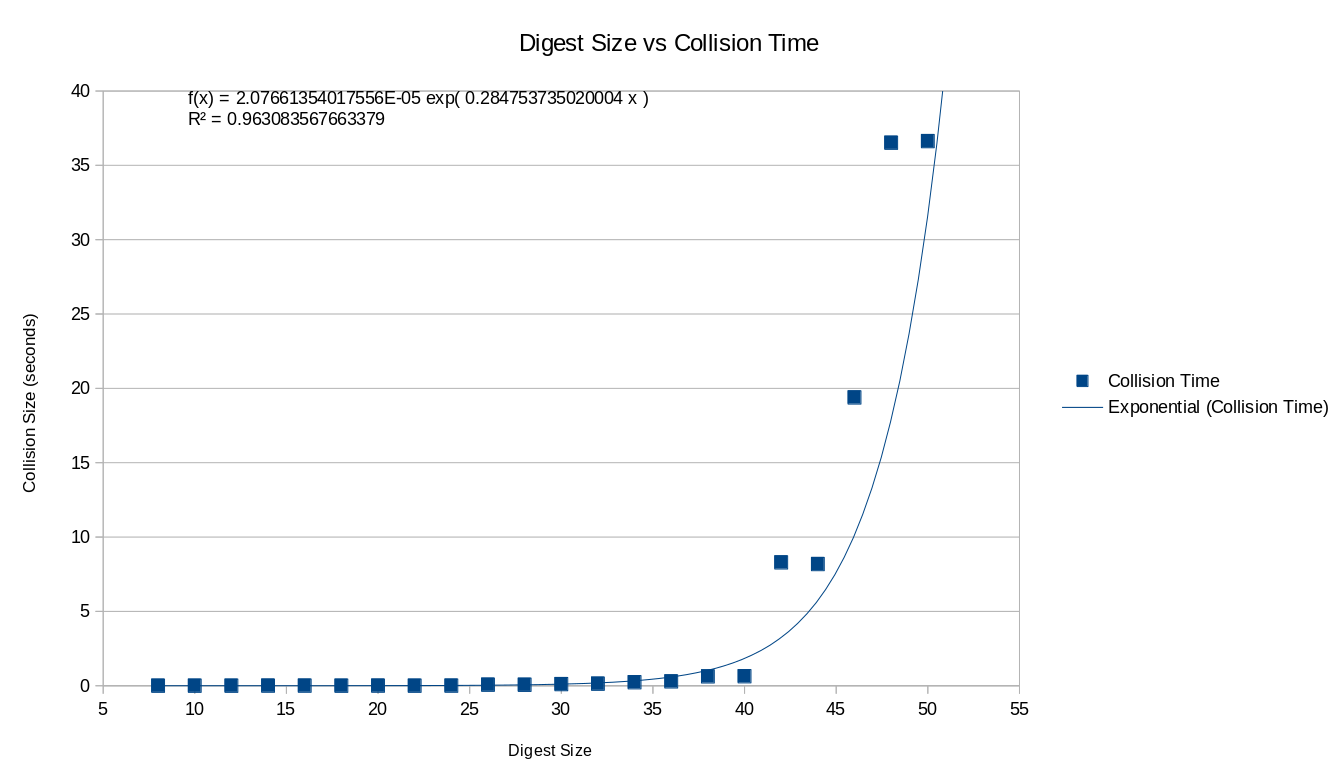
\includegraphics[width=18cm]{Images/D vs CT.png}
      \caption{Digest Size and Collision Time}
      \label{fig:D_v_CT}
    \end{figure}
\pagebreak

    \begin{figure}[h!]
      \centering
      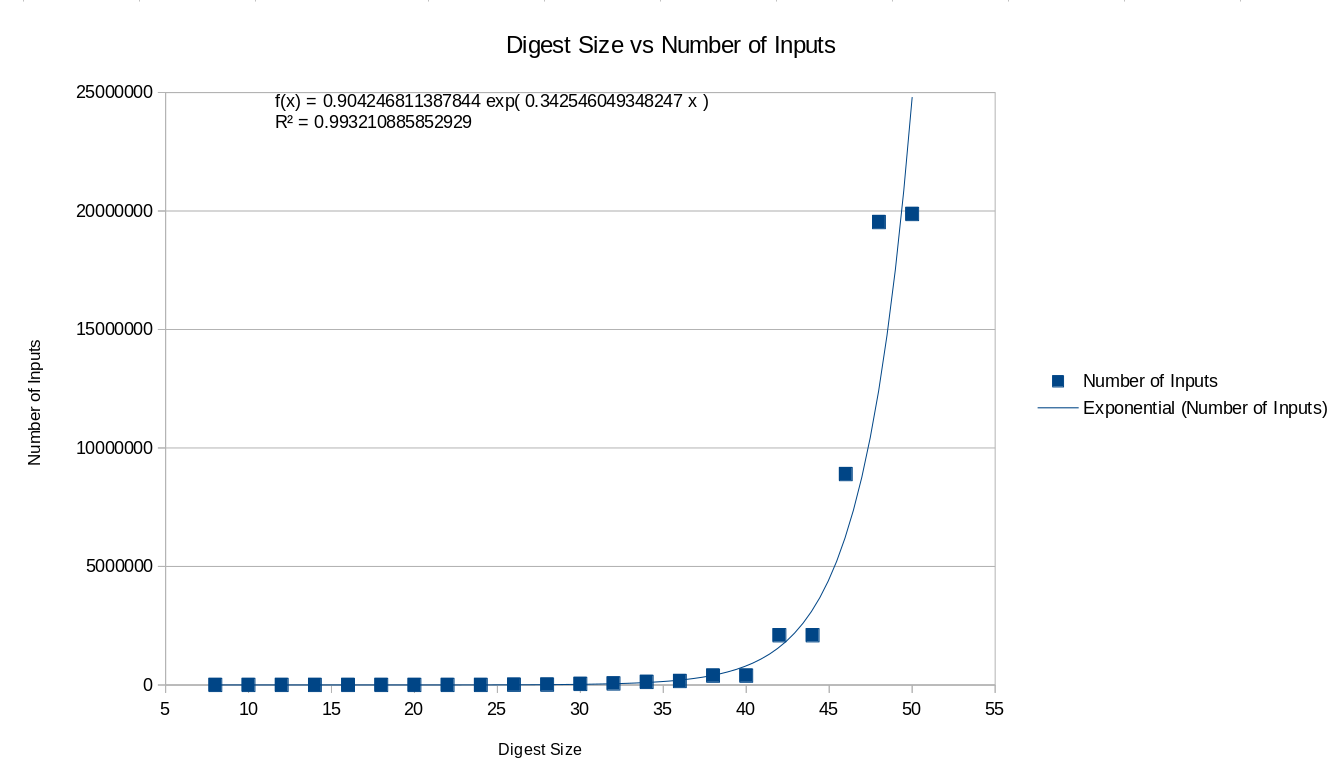
\includegraphics[width=18cm]{Images/D vs N o I.png}
      \caption{Digest Size and Number of Inputs}
      \label{fig:D_v_NoI}
    \end{figure}

\pagebreak
\section{Task 2}

  For this task, we are breaking bcrypt password hashes of varying 
  workfactors and salts with known password characteristics. Fortunately, 
  the password length is known to be between 6 and 10 characters and random 
  word from the ntlk word corpus. This produces about 135,000 possible words 
  that can be the password for each bcrypt hash. Additionally, we opted to 
  sort this list based upon length in hopes of shorter passwords being used.

  Overall, our script is successful and produced all of the passwords
  corresponding to the hashes. However, it is a very time intensive task 
  for hashes of workfactor 10+. We made some optimizations, such as cracking 
  passwords simultaneously that share the same salt. Further optimizations we 
  wanted to implement were multiprocessing, especially in relation to CUDA/utilizing 
  a GPU. The total runtime of this script on an Intel i7-8565U (mobile laptop CPU) 
  was approximately 13 hours. With multiprocessing this time could be greatly 
  decreased.

  \subsection{Code}
    \lstinputlisting[language=Python]{../task2.py}
  \subsection{Supplied Hashes}
    \lstinputlisting{../shadow.txt}
  \subsection{Usage}
    {\tt\begin{tabbing}                                                                                                                                                                     
       \$ pip3 install progressbar nltk\\
       \$ python3 task2.py \\
      \end{tabbing}}
  \subsection{Results}
    \lstinputlisting{../passwords.txt}

\pagebreak
\section{Questions}

  \subsection{What did you observe based on Task 1b? How many bytes are different
  between two digests?}

      In Task 1b, with inputs that had a hamming distance of 1, we noticed 
      that the digests that were produced were drastically different. 
      It seemed that all 32 bytes were different with no way of telling 
      that the two inputs were similar.

  \subsection{What is the maximum number of files you would ever need to hash 
  to find a collision of an n-bit digest? Given the birthday bound, what is the 
  expected number of hashes before a collision on an n-bit digest? Is this what
  you observed? Based on the data you have collected, speculate on how long it 
  might take to find a collision on the full 256-bit digest.}

      In order to find a hash collision of an n-bit digest, you would need 
      need a maximum of $2^n + 1$ files. Given the birthday bound, you would
      also need $2^n + 1$ hashes before a collision of an n-bit digest. In our 
      case, it was often much less to achieve a collision. If we use the 
      equation on our graph, it would take approximately
      $ 1.0974 * 10^{38}$ different values 
      to find a hash collision. This is much smaller than $2^{256} + 1$ 
      inputs that are required to find a collision. At a max rate of 8192.0 MH/s
      on an Nvidia GTX 3080 (according to the hashcat forums), it would still
      take about $1.3395*10^{28}$ seconds, or about $4.249 * 10^{20} $ years.

  \subsection{Given an 8-bit digest, would you be able to break the one-way 
  property (i.e. can you find any pre-image)? Do you think this would be 
  easier or harder than finding a collision? Why or why not?}

      Given an 8-bit digest, you could easily break the one-way property 
      of SHA-256. This is technically harder to do than just finding a
      collision due to the nature of hashing, however. If you were just trying 
      to find any collision you could systematically hash $2^8 + 1$ different 
      values until one of them yields in a collision. This is different from 
      finding a pre-image for a specific digest due to the collision resistant 
      nature of SHA-256. While it likely wouldn't take much more than $2^8 + 1$ 
      different inputs, it could take exponentially more if you are unlucky.

  \subsection{For Task 2, given your results, how long would it take to brute 
  force a password that uses the format word1:word2 where both words are
  between 6 and 10 character? What about word1:word2:word3? What about
  word1:word2:number where number is between 1 and 5 digits? Make sure to 
  sufficiently justify your answers.}
      Using the nltk corpus as our wordlist, if the format of the password 
      was word1:word2, we would have approximately $135,000 * 135,000 = 18,225,000,000$ different
      possible combinations. Assuming a workfactor of 8 and same amount of 
      compute power and single threaded program, it would take approximately
      $8*18,225,000,000/135,000 = 1,080,000$ minutes, or approximately 
      2.05 years. However, if you were to parallelize the hashing with 
      use of a GPU, this time could be drastically reduced, to the point of 
      being possible in a reasonable amount of time.

      Using the nltk corpus as our wordlist, if the format of the password 
      was word1:word2:word3, we would have approximately 
      $135,000 * 135,000 * 135,000= 2.46*10^{15}$ different
      possible combinations. Assuming a workfactor of 8 and same amount of 
      compute power and single threaded program, it would take approximately
      $8*2.46*10^{15}/135,000 = 145,800,000,000$ minutes, or approximately 
      277,397 years. However, if you were to parallelize the hashing with 
      use of a GPU, this time could be drastically reduced. 

      Using the nltk corpus as our wordlist, if the format of the password 
      was word1:word2:number, we would have approximately 
      $135,000 * 135,000 * 5 = 91,125,000,000$ different
      possible combinations. Assuming a workfactor of 8 and same amount of 
      compute power and single threaded program, it would take approximately
      $8*91,125,000,000/135,000 = 5,400,000$ minutes, or approximately 
      10.27 years. However, if you were to parallelize the hashing with 
      use of a GPU, this time could be drastically reduced, to the point of 
      being possible in a more reasonable amount of time.

\end{document}
